\begin{figure}[t]
\centering
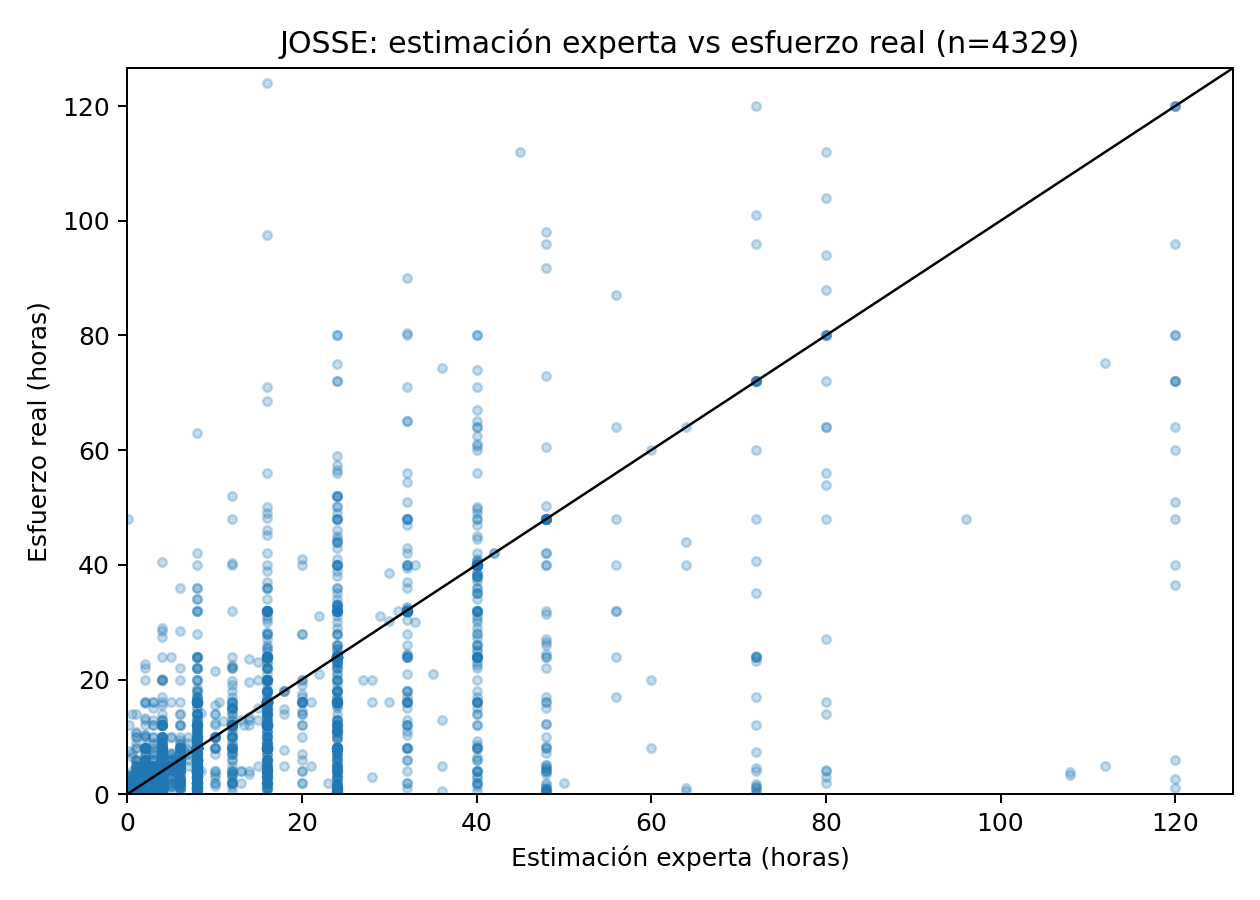
\includegraphics[width=0.95\linewidth]{../outputs/figures/josse_expert_vs_actual.png}
\caption{Estimaci\'on experta contra esfuerzo real en JOSSE. La l\'inea diagonal indica estimaci\'on perfecta.}
\label{fig:expertos}
\end{figure}

\begin{figure}[t]
\centering
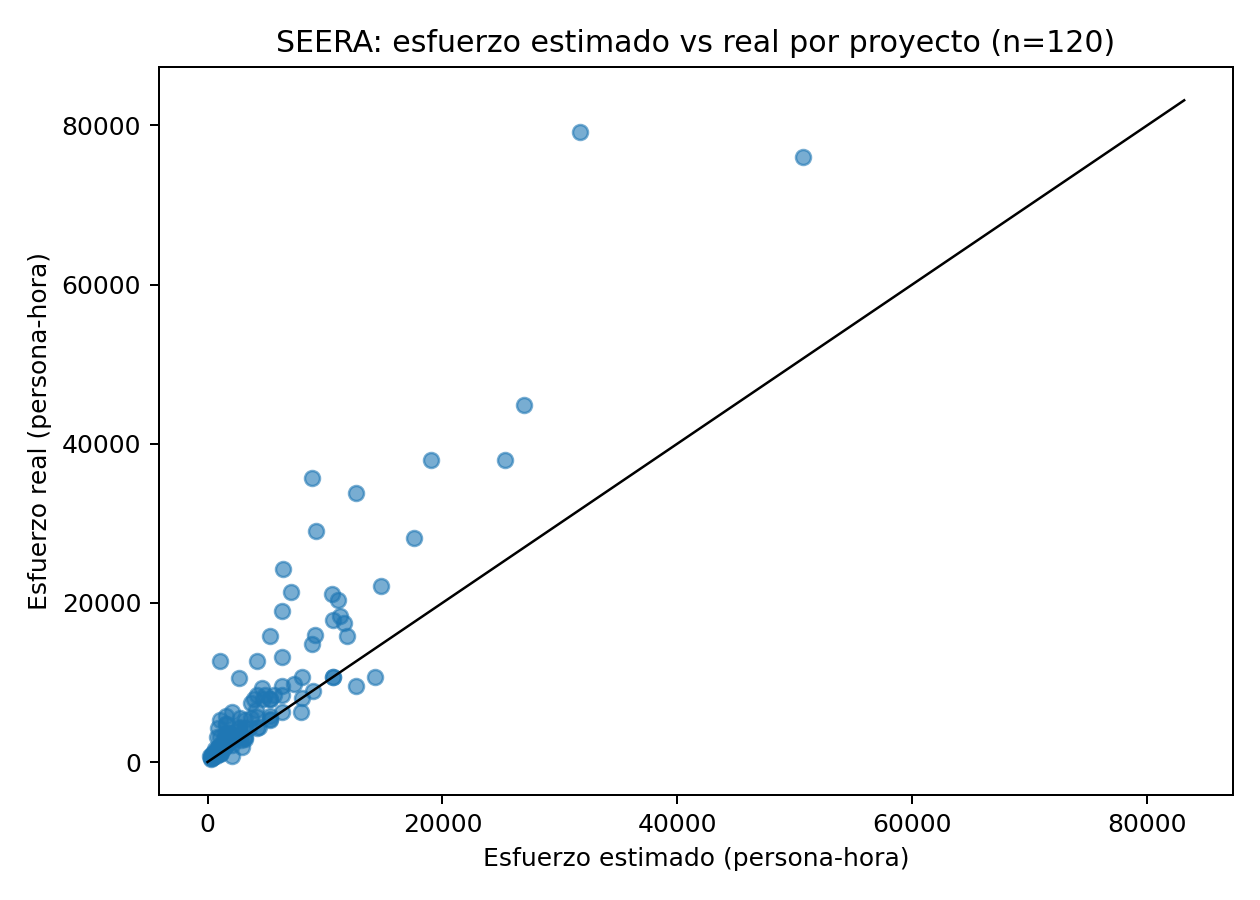
\includegraphics[width=0.95\linewidth]{../outputs/figures/seera_estimate_vs_actual.png}
\caption{Esfuerzo estimado contra esfuerzo real por proyecto en SEERA. Los puntos por encima de la diagonal corresponden a proyectos subestimados.}
\label{fig:seera}
\end{figure}

\begin{figure}[t]
\centering
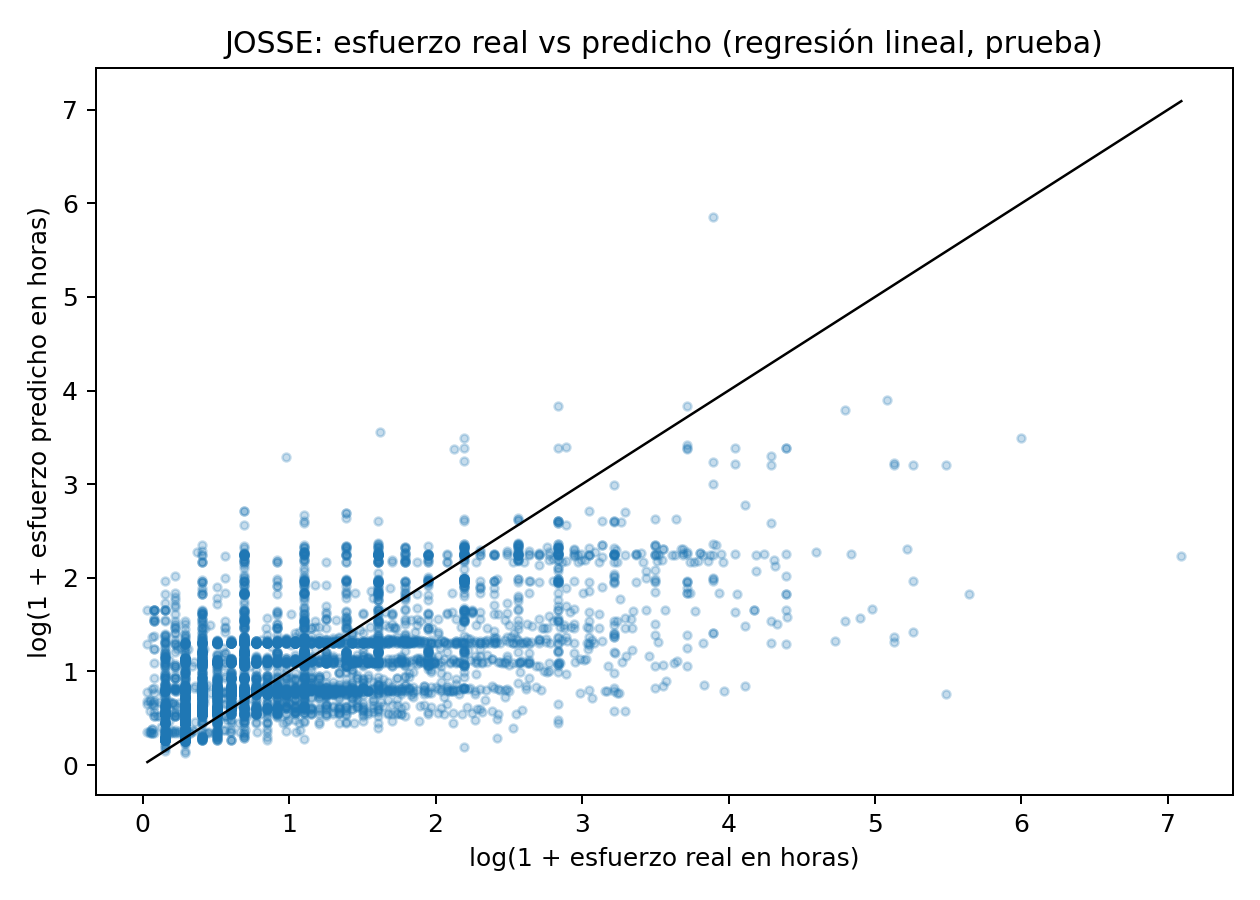
\includegraphics[width=0.95\linewidth]{../outputs/figures/actual_vs_predicted_josse.png}
\caption{Esfuerzo real contra esfuerzo predicho por la regresi\'on lineal en el conjunto de prueba de JOSSE.}
\label{fig:pred}
\end{figure}

\begin{figure}[t]
\centering
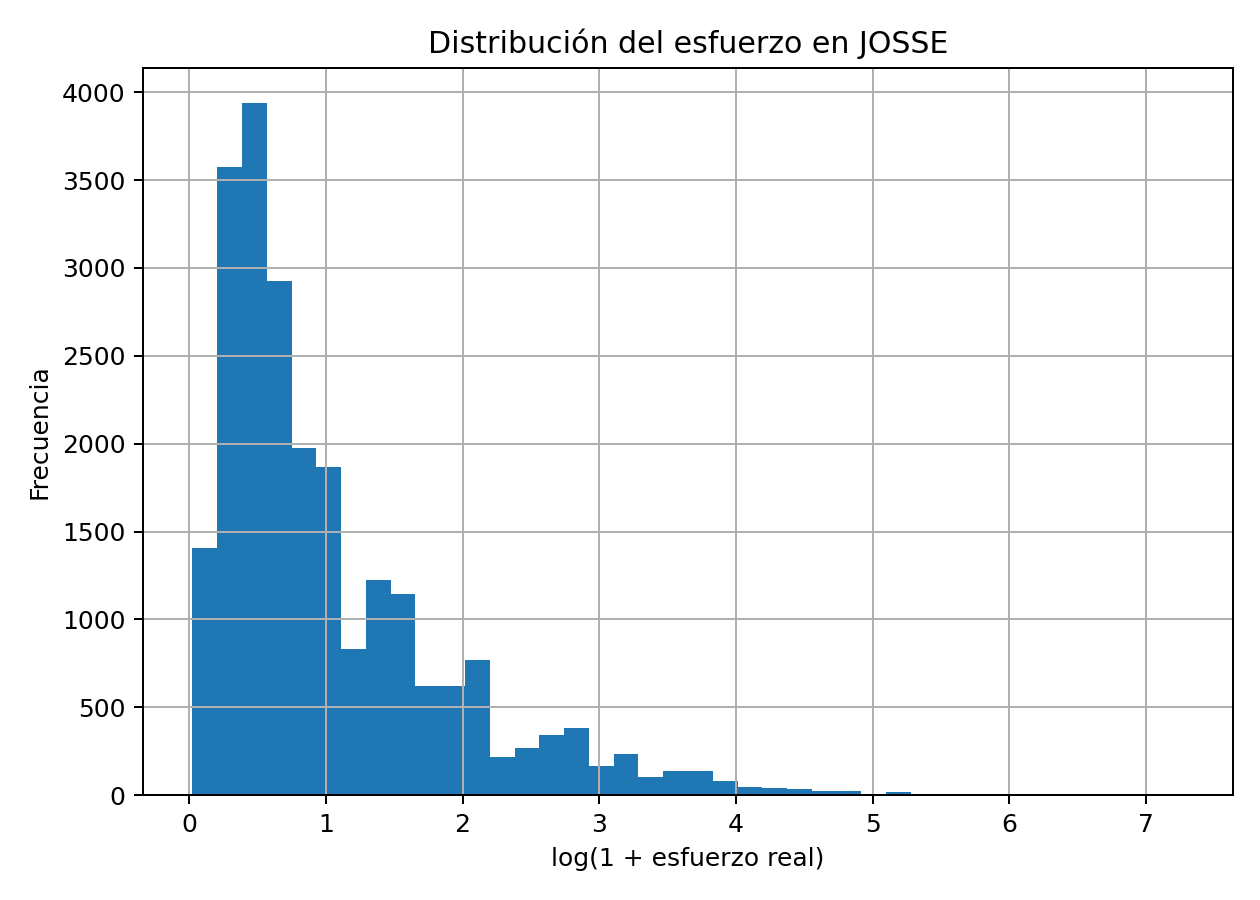
\includegraphics[width=0.95\linewidth]{../outputs/figures/effort_distribution_josse.png}
\caption{Distribuci\'on del esfuerzo real en JOSSE (escala logar\'itmica).}
\label{fig:distjosse}
\end{figure}

\begin{figure}[t]
\centering
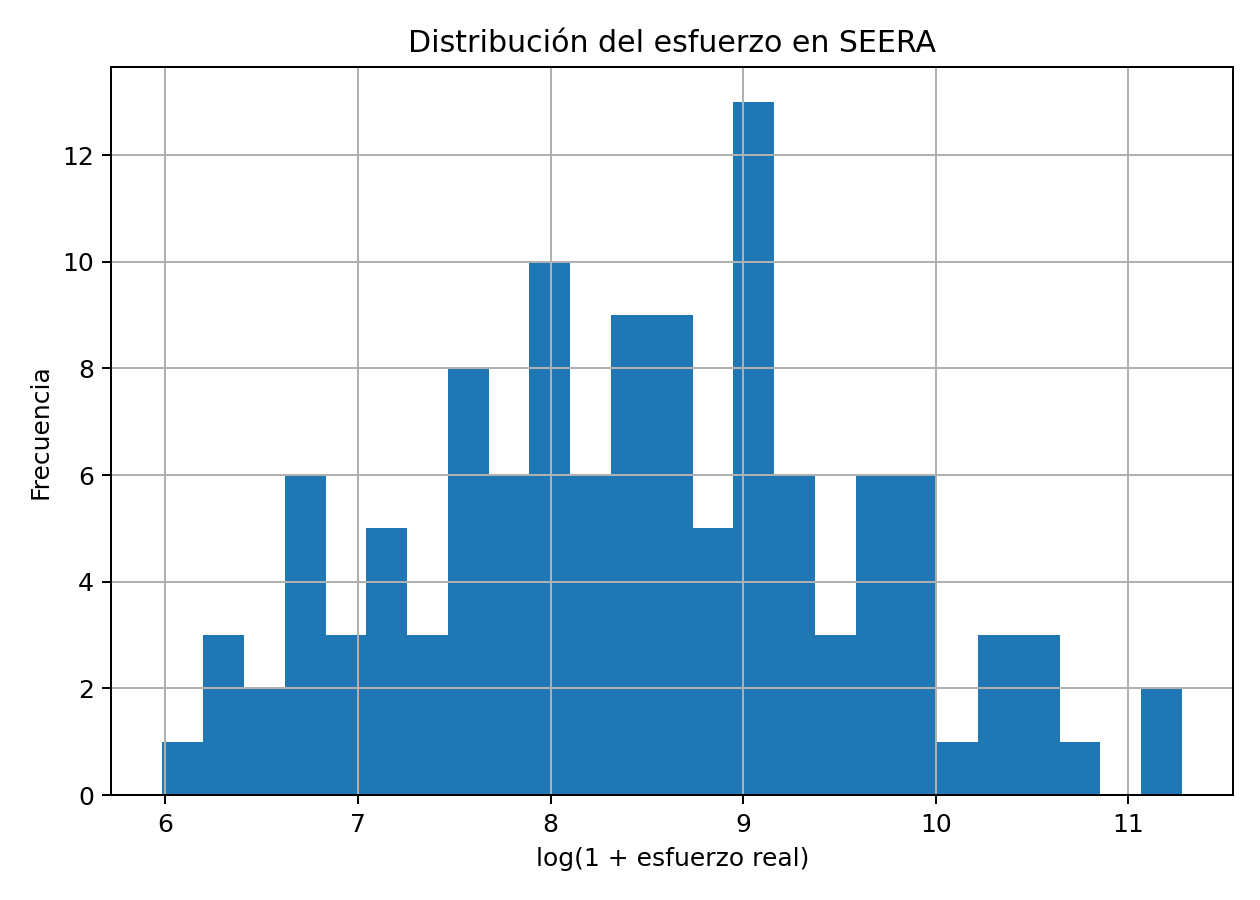
\includegraphics[width=0.95\linewidth]{../outputs/figures/effort_distribution_seera.png}
\caption{Distribuci\'on del esfuerzo real en SEERA (escala logar\'itmica).}
\label{fig:distseera}
\end{figure}

\begin{figure}[t]
\centering
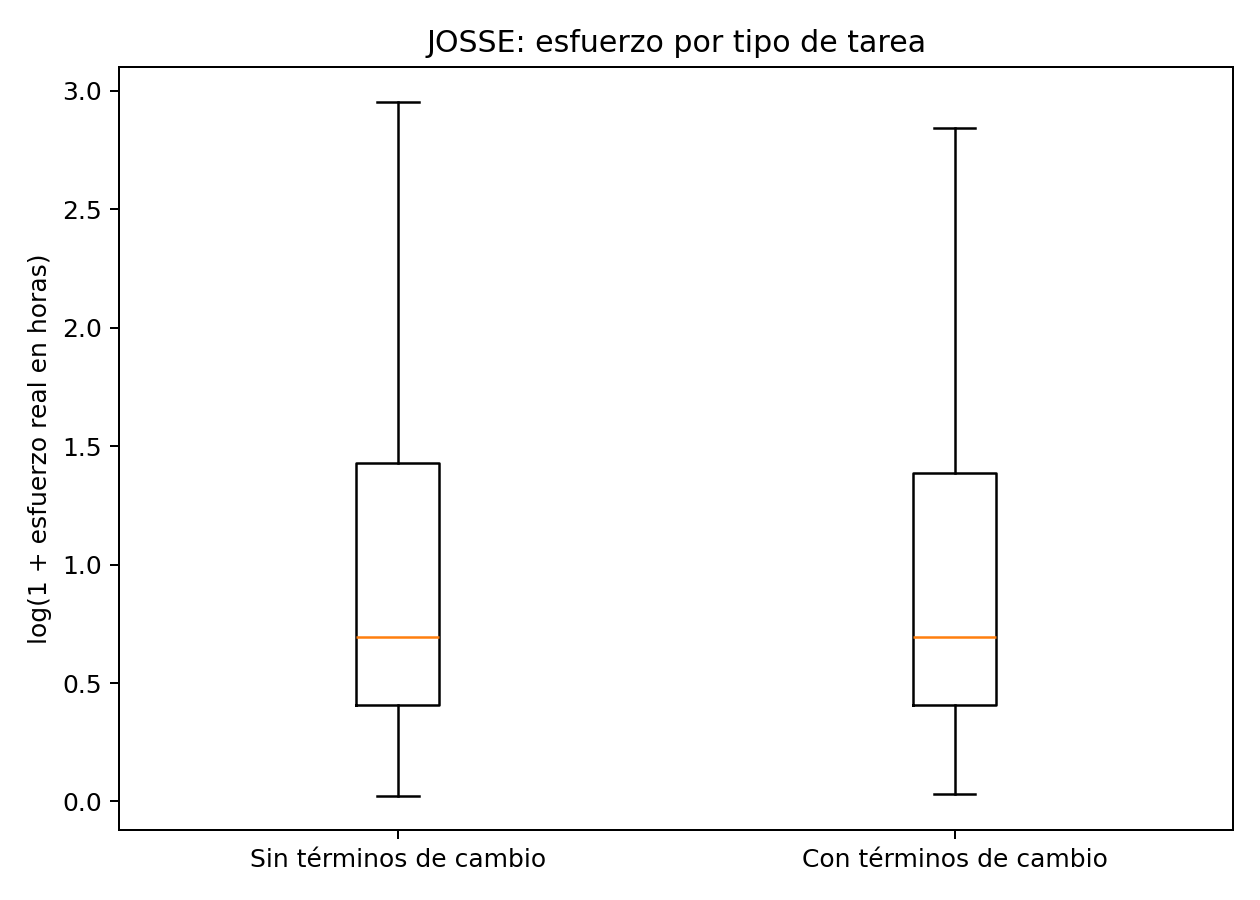
\includegraphics[width=0.95\linewidth]{../outputs/figures/josse_change_boxplot.png}
\caption{Esfuerzo real por tipo de tarea en JOSSE (sin valores at\'ipicos).}
\label{fig:boxplot}
\end{figure}
